\subsection{Wechselstrom-Schalter/Steller}
\subsubsection{Wechselstrom-Schalter}
\begin{minipage}{\linewidth}
    Wegen dem Polaritätswechel besteh der Wechselstromschalter aus zwei antiparallelen Thyristoren, welche die Stromhalbschwingung abwechselnd ausführen.
\end{minipage}

\begin{minipage}{0.3\linewidth}
    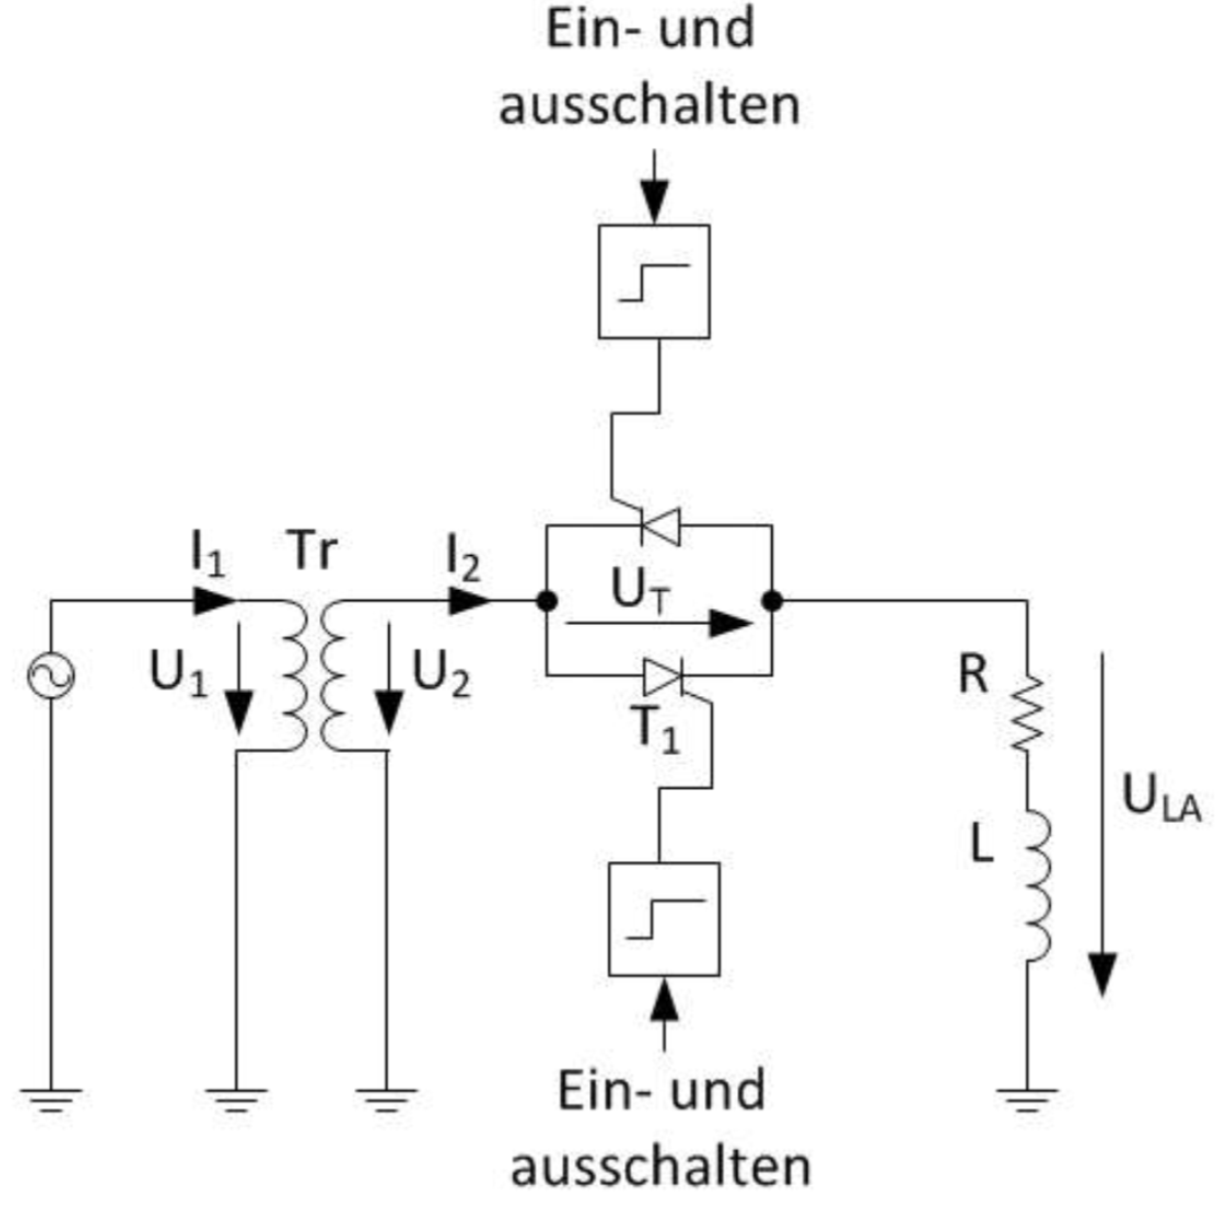
\includegraphics[width=\linewidth]{images/SchemaWSSchalter}
\end{minipage}
\begin{minipage}{0.3\linewidth}
    \textbf{Lasttyp: R}\newline
    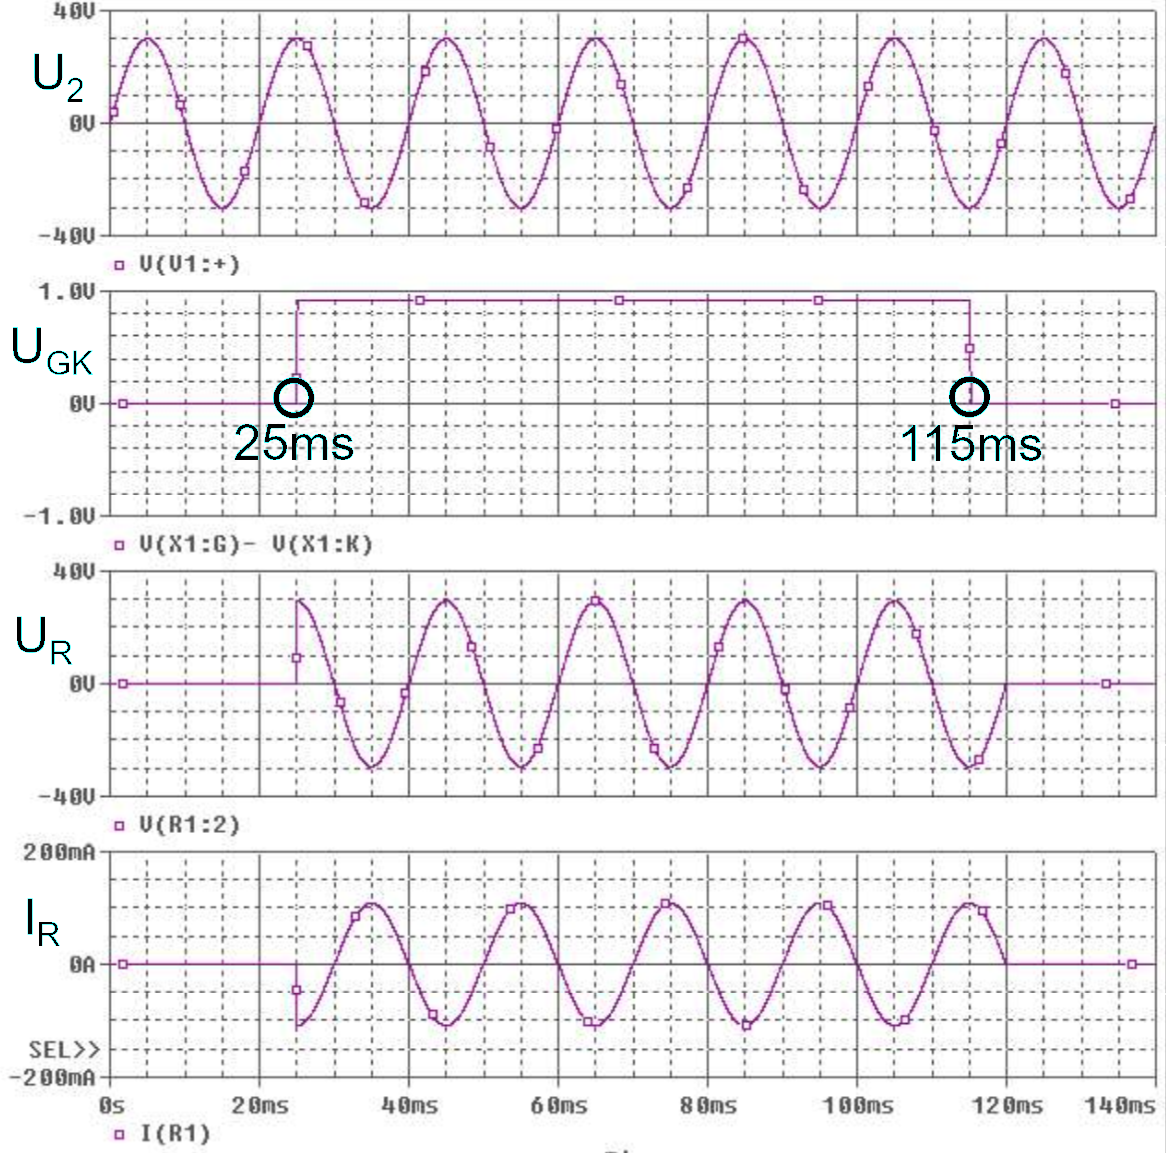
\includegraphics[width=\linewidth]{images/KLWSSchalter}
\end{minipage}
\begin{minipage}{0.3\linewidth}
    \textbf{Lasttyp: R + L}\newline
    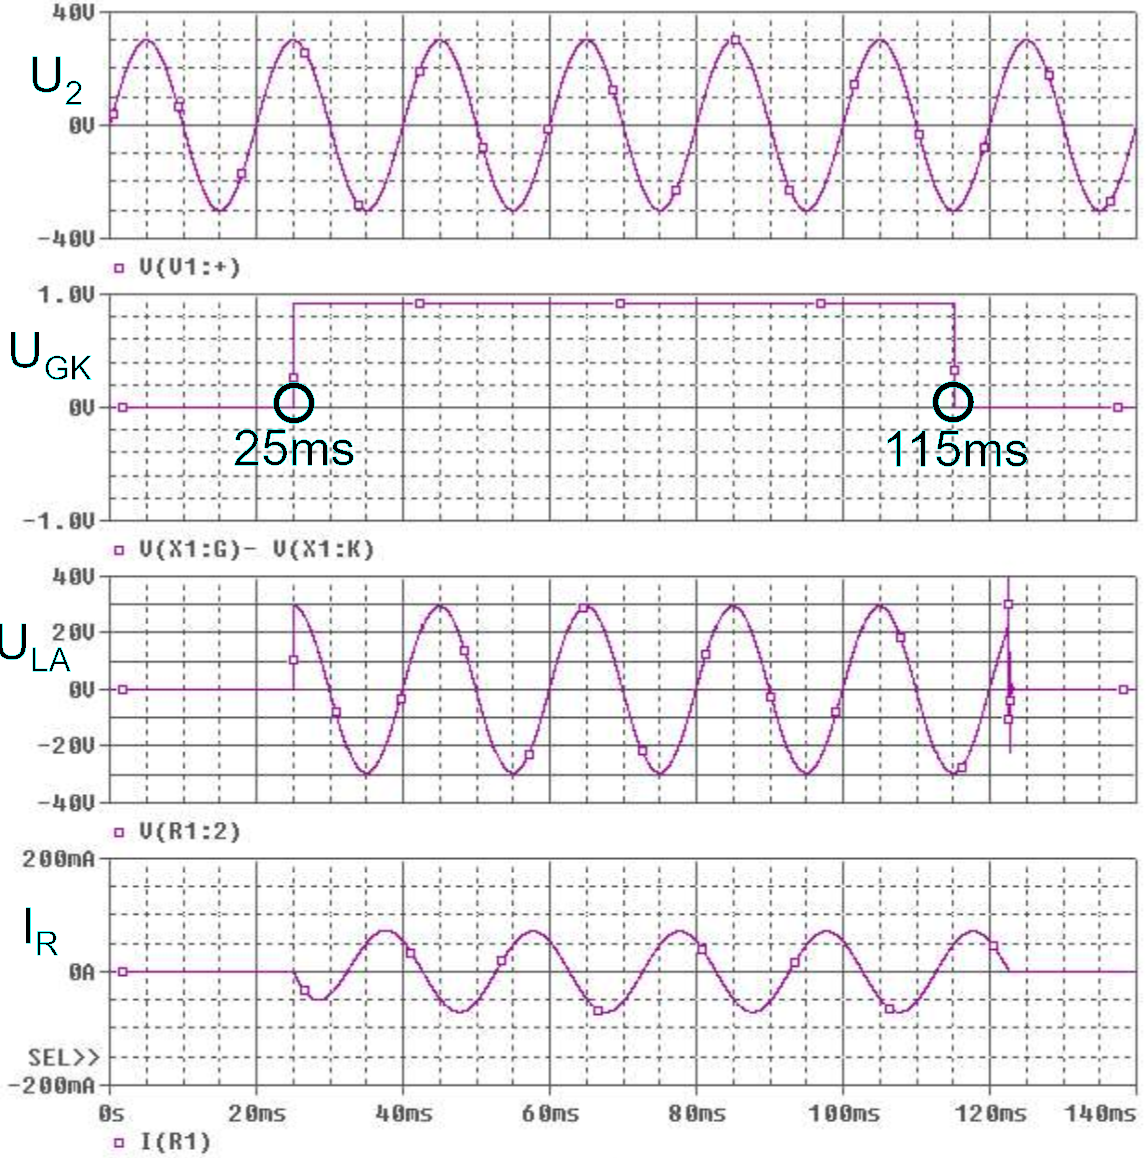
\includegraphics[width=\linewidth]{images/KLWSSchalter2}
\end{minipage}

\subsubsection{Wechselstrom-Steller}
\begin{minipage}{\linewidth}
    Im vergleich mit den Wechselstrom-Schalter, welche eimaligs Ein- oder Ausschalten von Wechselstromkreisen ermöglichen, erlaubt der Wechselstrom-Steller in jeder Halbperiode wiederholtes Einschalten, wobei der Strom vom Zündzeitpunkt bis zm Nulldurchgang fliesst.
\end{minipage}

\begin{minipage}{0.3\linewidth}
    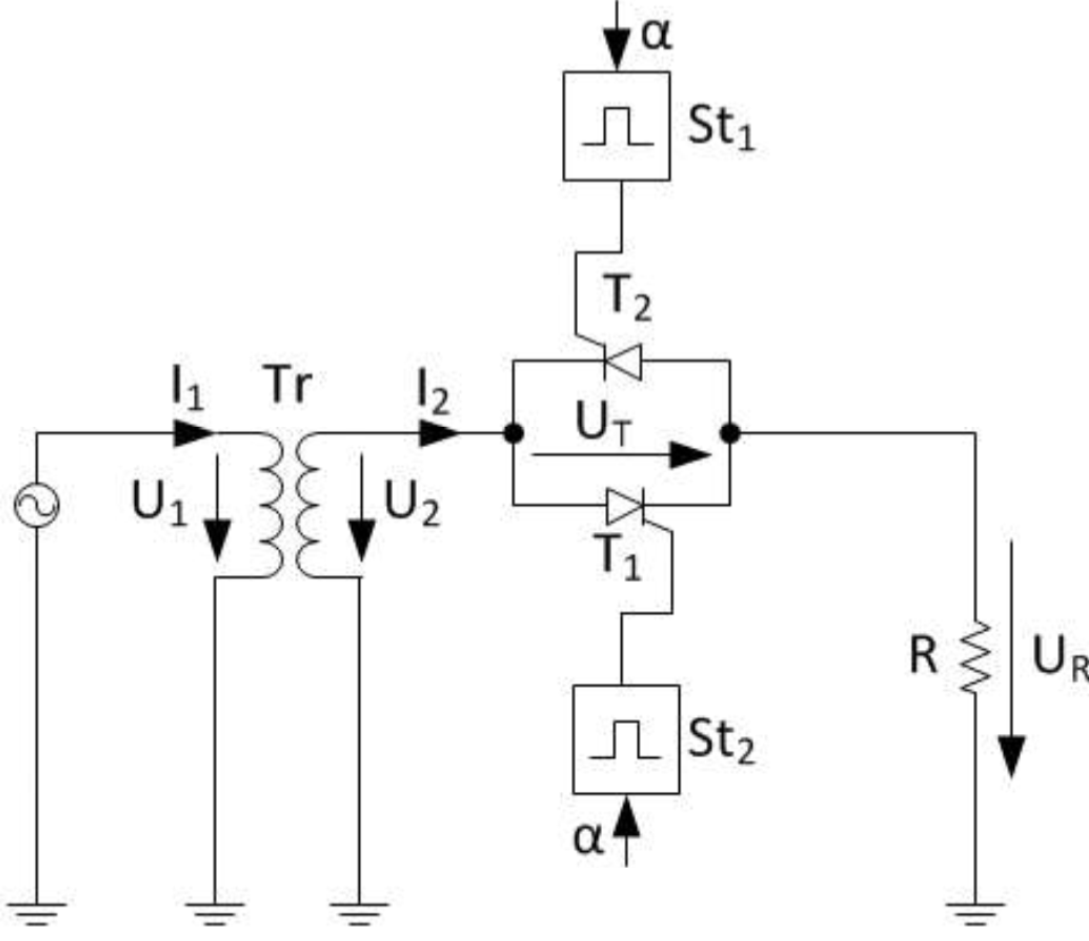
\includegraphics[width=\linewidth]{images/SchemaWSSteller}
\end{minipage}
\begin{minipage}{0.3\linewidth}
    \textbf{Lasttyp: R}\newline
    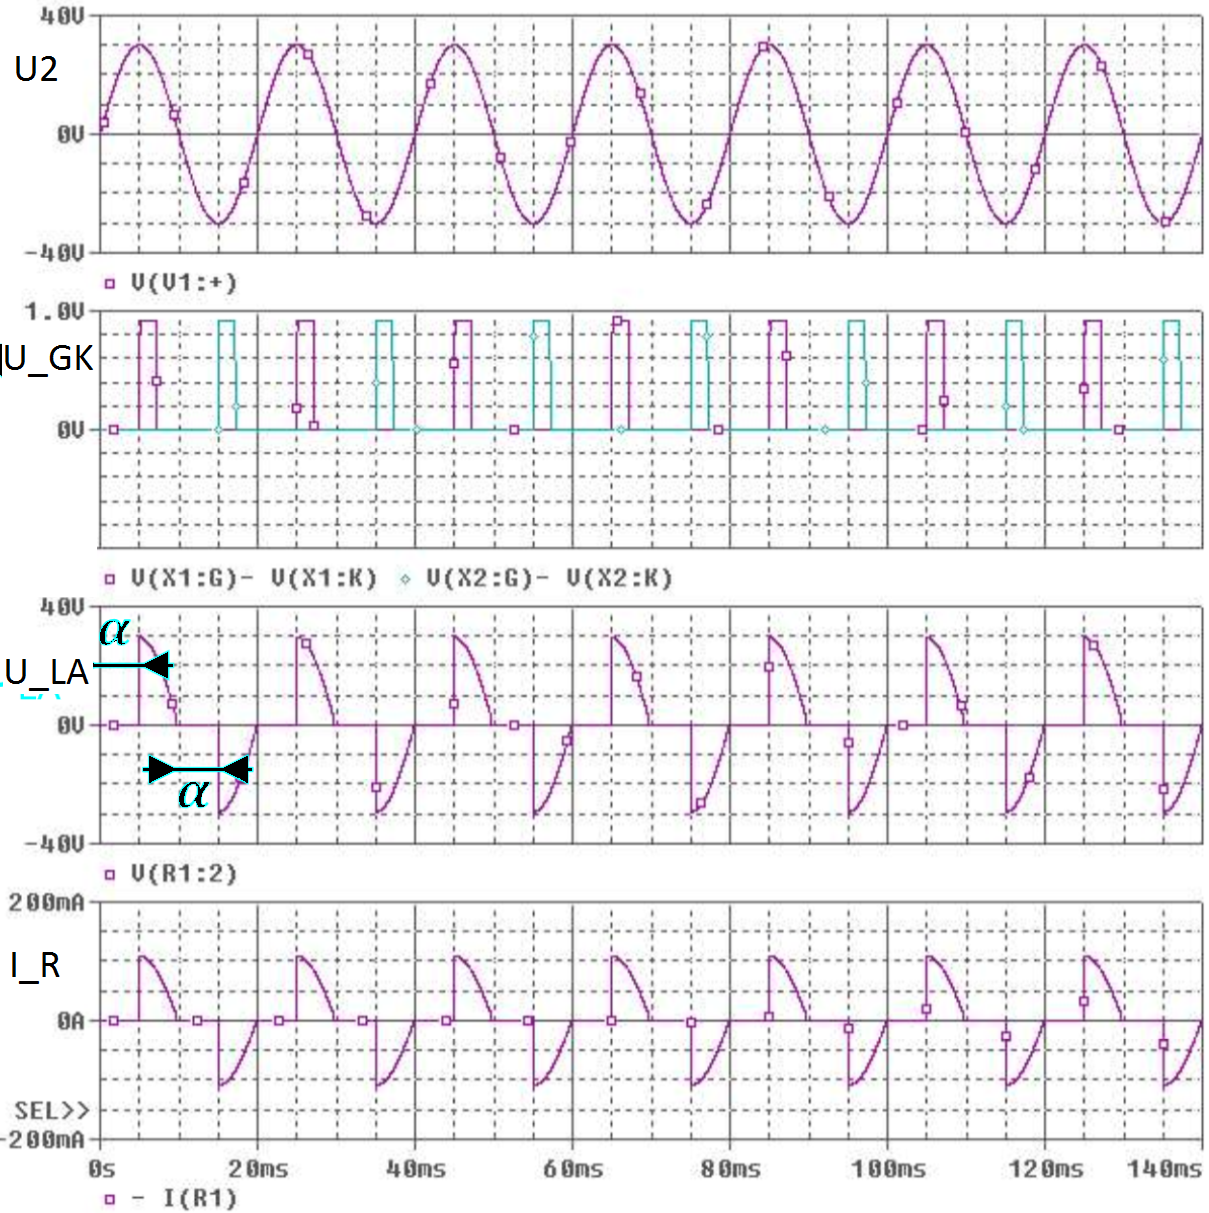
\includegraphics[width=\linewidth]{images/KLWSSteller}
\end{minipage}
\begin{minipage}{0.3\linewidth}
    \textbf{Lasttyp: R + L}\newline
    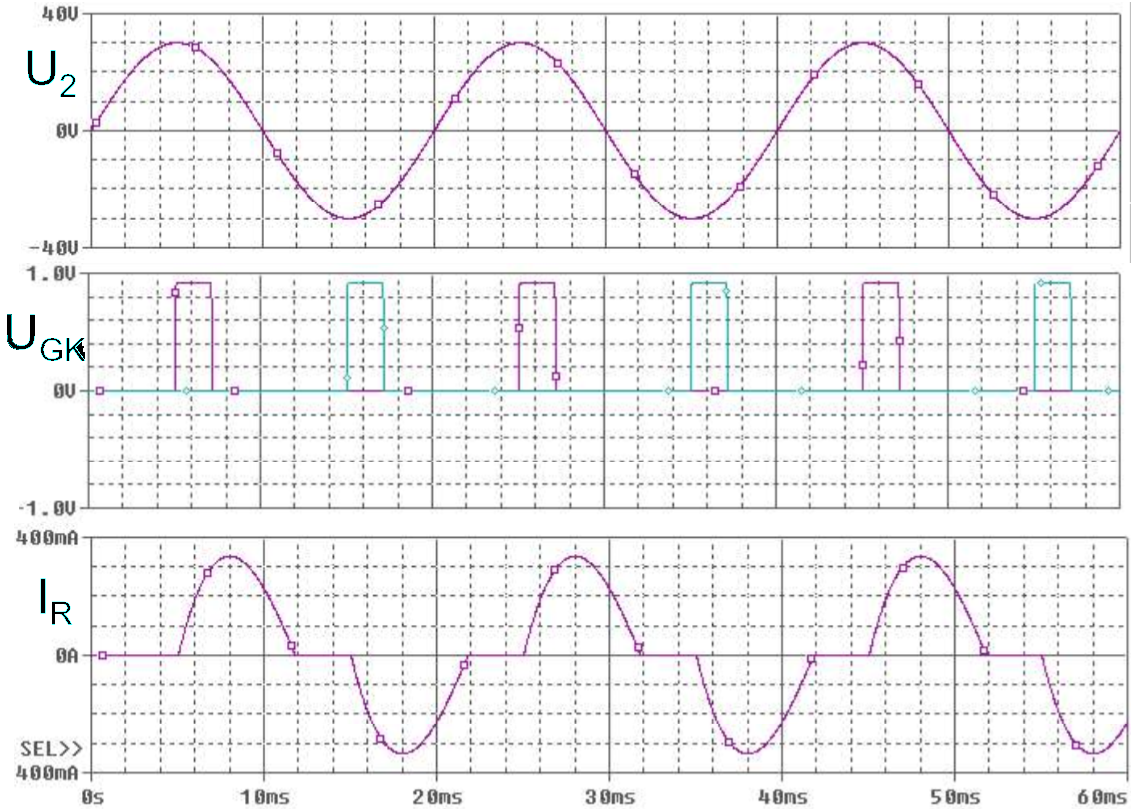
\includegraphics[width=\linewidth]{images/KLWSSteller2}
\end{minipage}

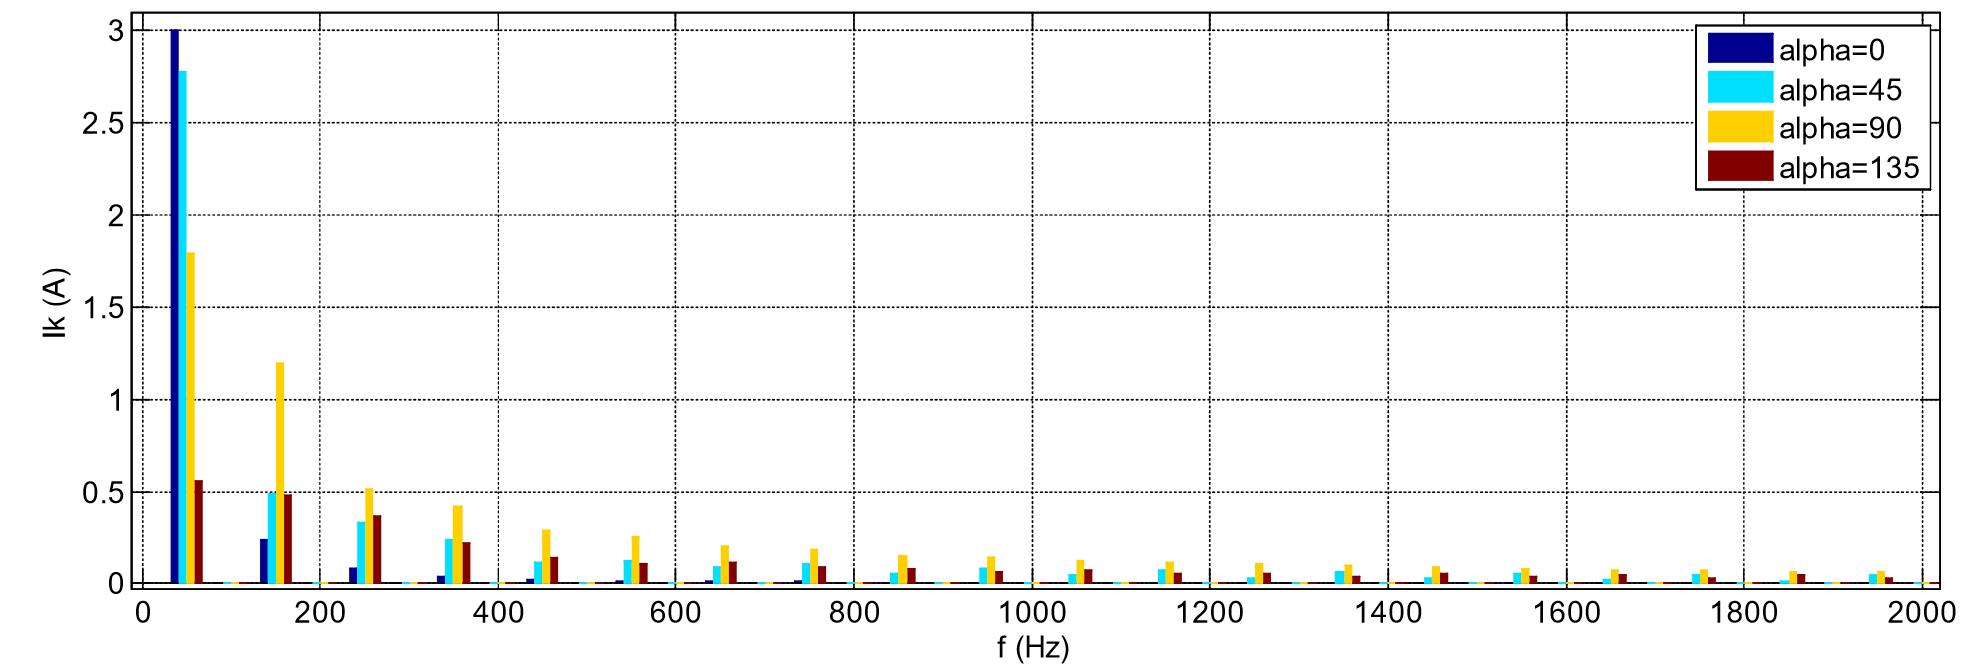
\includegraphics[width=\linewidth]{images/OWWSSteller}

%\begin{minipage}{0.3\linewidth}
%    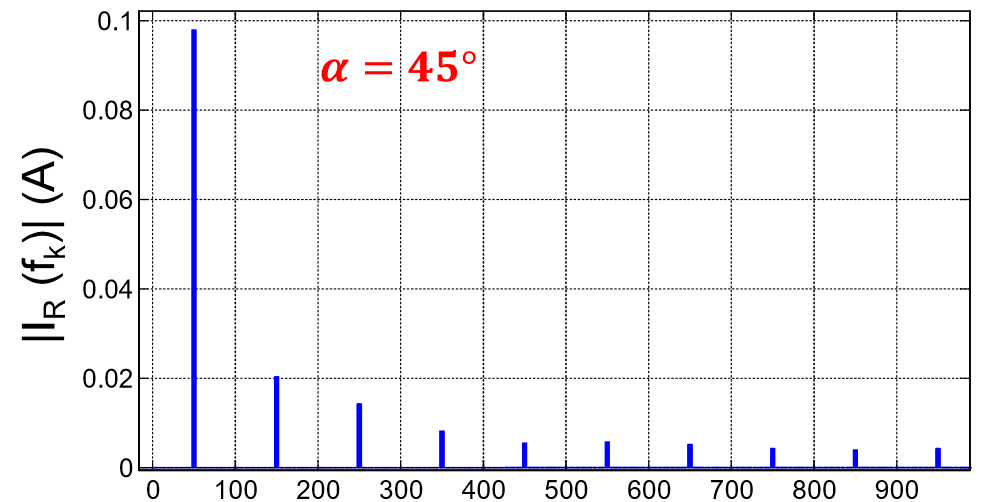
\includegraphics[width=\linewidth]{images/OW45WSSteller}
%    
%    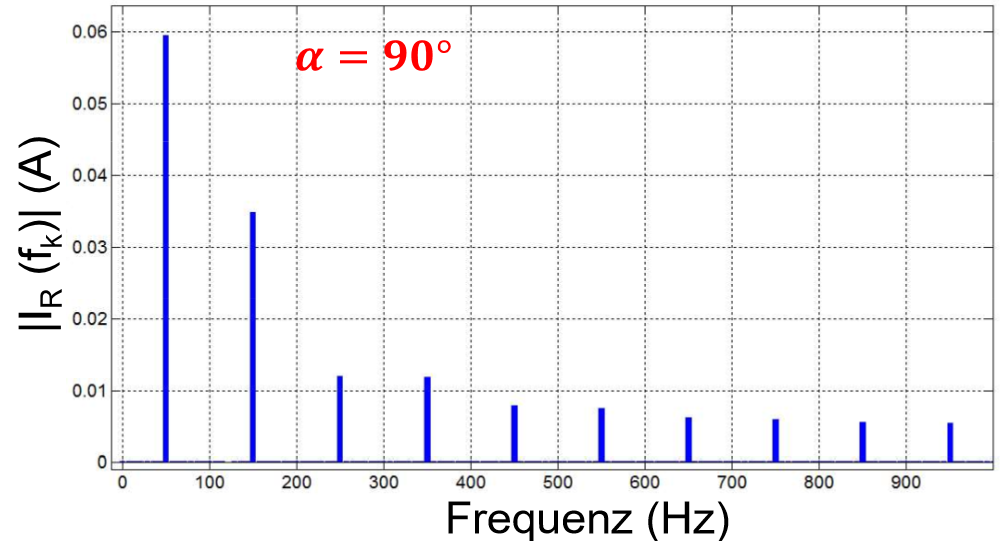
\includegraphics[width=\linewidth]{images/OW90WSSteller}
%\end{minipage}
\clearpage